\documentclass[conference]{IEEEtran}
\IEEEoverridecommandlockouts
\usepackage{cite}
\usepackage{amsmath,amssymb,amsfonts}
\usepackage{algorithmic}
\usepackage{graphicx}
\usepackage{textcomp}
\usepackage{xcolor}
\usepackage{booktabs}
\usepackage{multirow}
\usepackage{url}
\usepackage[hidelinks]{hyperref}
\usepackage{listings}
\usepackage{float}

% Code listing style
\lstset{
  basicstyle=\ttfamily\tiny,
  breaklines=true,
  frame=single,
  language=Python,
  showstringspaces=false
}

\def\BibTeX{{\rm B\kern-.05em{\sc i\kern-.025em b}\kern-.08em
    T\kern-.1667em\lower.7ex\hbox{E}\kern-.125emX}}

\begin{document}

\title{Fine-tuning Language Models for Code Translation and Generation: A Comparative Study of Full Parameter and LoRA Approaches}

\author{\IEEEauthorblockN{Shujun Liao}
\IEEEauthorblockA{ge83juz@tum.de \\
\textit{Technical University of Munich}\\
Heilbronn, Baden-Württemberg, Germany}
\and
\IEEEauthorblockN{Vipin Chaudhry}
\IEEEauthorblockA{go98vib@mytum.de \\
\textit{Technical University of Munich}\\
Heilbronn, Baden-Württemberg, Germany}
}

\maketitle

\begin{abstract}
This paper presents a comprehensive study on fine-tuning large language models for code-related tasks, specifically focusing on cross-language code translation and code generation. We investigate two distinct fine-tuning approaches: full parameter fine-tuning and Low-Rank Adaptation (LoRA). For code translation, we fine-tune CodeT5 on the XLCoST dataset for Java to C\# translation, achieving a BLEU score improvement from 54.17 to 100.00, CodeBLEU from 0.1029 to 0.9390, and a functional correctness rate of 72.06\%. For code generation, we apply LoRA fine-tuning to deepseek-coder-6.7b-instruct and Qwen2.5-Coder-3B-Instruct models for Python code synthesis from natural language descriptions. Our experiments demonstrate that LoRA enables efficient fine-tuning with only 1-2\% trainable parameters while achieving competitive performance. DeepSeek Coder shows significant improvement with Pass@1 increasing from 39.70\% to 57.00\%, while Qwen achieves even larger gains from 33.55\% to 61.20\%. Both models show dramatic reductions in syntax and runtime errors after LoRA fine-tuning. Our findings provide insights into the trade-offs between full fine-tuning and parameter-efficient methods for code intelligence tasks.
\end{abstract}

\begin{IEEEkeywords}
Code Translation, Code Generation, Large Language Models, Fine-tuning, LoRA, CodeT5, DeepSeek Coder, Qwen Coder
\end{IEEEkeywords}

\section{Introduction}

The emergence of large language models (LLMs) has revolutionized the field of software engineering, enabling automated code generation, translation, and analysis at unprecedented levels of quality~\cite{chen2021codex}. As software systems become increasingly complex and multilingual, the ability to automatically translate code between programming languages and generate functional code from natural language specifications has become crucial for developer productivity and software maintenance.

Code translation, the task of converting source code from one programming language to another while preserving functionality, addresses critical challenges in software migration and modernization. Organizations frequently need to migrate legacy systems from older languages to modern platforms, a process that is traditionally manual, error-prone, and expensive. The Java to C\# translation task is particularly relevant given the widespread adoption of both languages in enterprise environments and their syntactic similarities that make neural translation feasible.

Similarly, code generation from natural language descriptions has the potential to democratize software development by allowing developers to express their intent in plain language rather than detailed syntax. This capability is especially valuable for rapid prototyping, educational purposes, and assisting developers with unfamiliar APIs or algorithms.

Pre-trained code models such as CodeT5~\cite{wang2021codet5}, CodeBERT~\cite{feng2020codebert}, and more recent decoder-only models like DeepSeek Coder~\cite{deepseek2024} and Qwen2.5 Coder~\cite{qwen2024} have shown impressive capabilities on various code understanding and generation tasks. However, these models typically require task-specific fine-tuning to achieve optimal performance on downstream applications.

Fine-tuning approaches can be broadly categorized into two paradigms: full parameter fine-tuning and parameter-efficient fine-tuning (PEFT). Full fine-tuning updates all model parameters and often achieves the best task-specific performance but requires significant computational resources. In contrast, PEFT methods such as Low-Rank Adaptation (LoRA)~\cite{hu2021lora} update only a small fraction of parameters while maintaining competitive performance, making them attractive for resource-constrained environments.

In this paper, we present a comparative study of these two fine-tuning approaches applied to code translation and code generation tasks. Our main contributions are:

\begin{itemize}
    \item We demonstrate that full fine-tuning of CodeT5 (222.88M parameters) on the XLCoST dataset achieves state-of-the-art performance on Java to C\# translation, with BLEU scores improving by 84.6\%, CodeBLEU by 813\%, and functional correctness reaching 72.06\%.
    
    \item We evaluate LoRA fine-tuning on two modern code LLMs (deepseek-coder-6.7b-instruct and Qwen2.5-Coder-3B-Instruct) for Python code generation, showing that training only 1.13-1.73\% of parameters can yield significant improvements in Pass@1 metrics and dramatically reduce syntax errors.
    
    \item We provide a comprehensive analysis comparing full fine-tuning and LoRA approaches in terms of training efficiency, resource requirements, error distribution, and downstream task performance.
    
    \item We present detailed error analysis and code quality metrics, illustrating common failure patterns and the impact of fine-tuning on code style and correctness.
\end{itemize}

\section{Related Work}

\subsection{Neural Code Translation}

Neural machine translation techniques have been successfully adapted for code translation tasks. TransCoder~\cite{roziere2020transcoder} pioneered unsupervised code translation using denoising auto-encoding and back-translation, demonstrating that large-scale pre-training on monolingual code corpora enables effective cross-language translation without parallel data. PLBART~\cite{ahmad2021plbart} extended BART to programming languages, achieving strong results on code translation benchmarks through unified pre-training on both natural language and code.

CodeT5~\cite{wang2021codet5} introduced identifier-aware pre-training objectives that help the model understand the semantic meaning of code tokens, particularly variable and function names. This approach proved especially effective for code translation tasks where preserving semantic relationships is crucial.

The XLCoST benchmark~\cite{xlcost2022} provides parallel code corpora across seven programming languages (C++, Java, Python, C\#, JavaScript, PHP, and C), enabling supervised training and evaluation of code translation models at both snippet and program levels.

\subsection{Code Generation from Natural Language}

Generating executable code from natural language descriptions has been a long-standing goal in software engineering research. Early approaches relied on semantic parsing and domain-specific languages, which were limited in scope and flexibility.

The advent of transformer-based models brought significant improvements, with models like Codex~\cite{chen2021codex} demonstrating remarkable code generation capabilities. GPT-4 and subsequent models have achieved even higher performance on code benchmarks, though they remain proprietary.

Recent open-source models such as StarCoder~\cite{starcoder2023}, DeepSeek Coder~\cite{deepseek2024}, and Qwen Coder~\cite{qwen2024} have achieved competitive performance with proprietary models. DeepSeek Coder is trained on 2 trillion tokens from 87 programming languages and demonstrates strong instruction-following capabilities. These models are pre-trained on large-scale code corpora and can be further fine-tuned for specific tasks.

The HumanEval benchmark~\cite{chen2021codex} introduced the Pass@k metric for evaluating functional correctness of generated code, which has become the standard evaluation protocol. This metric measures the probability that at least one of k generated samples passes all unit tests.

\subsection{Parameter-Efficient Fine-Tuning}

As language models grow in size, full fine-tuning becomes increasingly expensive in terms of both computation and memory. Parameter-efficient fine-tuning (PEFT) methods address this challenge by updating only a small subset of model parameters while keeping the majority frozen.

Adapter layers~\cite{houlsby2019adapters} insert small trainable modules between transformer layers, typically adding 1-5\% additional parameters. Prefix tuning~\cite{li2021prefix} prepends learnable tokens to the input, modifying the model's attention patterns without changing its weights.

Low-Rank Adaptation (LoRA)~\cite{hu2021lora} represents weight updates as low-rank decomposition matrices, enabling efficient fine-tuning with minimal additional parameters. For a weight matrix $W_0 \in \mathbb{R}^{d \times k}$, LoRA adds $\Delta W = BA$ where $B \in \mathbb{R}^{d \times r}$ and $A \in \mathbb{R}^{r \times k}$ with rank $r \ll \min(d, k)$.

QLoRA~\cite{dettmers2023qlora} combines LoRA with 4-bit quantization, allowing fine-tuning of models with billions of parameters on consumer-grade GPUs with as little as 8GB VRAM. This democratizes access to fine-tuning large models for academic and individual researchers.

\section{Methodology}

This section describes our two-part approach to code intelligence tasks: full parameter fine-tuning for code translation and LoRA-based fine-tuning for code generation.

\subsection{Implementation Pipeline}

We developed two integrated training pipelines for our experiments: \textbf{Kabul} for code translation and \textbf{LLMTrainPipeline} for code generation.

\subsubsection{Kabul: Code Translation Pipeline}
The Kabul pipeline implements a modular architecture for training and evaluating code translation models:

\begin{itemize}
    \item \textbf{Training Module} (\texttt{train\_model.py}): Orchestrates the fine-tuning process using HuggingFace's Seq2SeqTrainer with custom callbacks for detailed logging and progress reporting.
    \item \textbf{Evaluation Module} (\texttt{evaluate\_model.py}): Provides multidimensional evaluation including BLEU, CodeBLEU (with AST and DataFlow analysis), compilation testing via .NET SDK, and functional correctness verification.
    \item \textbf{Post-Processing Pipeline} (\texttt{post\_process.py}): Implements a three-layer cleaning pipeline: (1) Rule-based regex transformations for Java-to-C\# syntax mapping, (2) Code formatting via \texttt{dotnet format}, and (3) Compiler-aided self-healing using iterative error fixing.
\end{itemize}

\subsubsection{LLMTrainPipeline: Code Generation Pipeline}
The LLMTrainPipeline provides a comprehensive web-based interface for LoRA fine-tuning experiments:

\begin{itemize}
    \item \textbf{Training Service}: Executes QLoRA training with 4-bit quantization, supporting multiple model architectures (DeepSeek, Qwen, LLaMA). Includes automatic checkpoint management and real-time loss monitoring.
    \item \textbf{Evaluation Service}: Implements Pass@k evaluation with sandboxed code execution, syntax validation, and detailed error categorization.
    \item \textbf{Post-Processing}: Handles output format normalization through a registry-based system that adapts to different model output styles (function-only, competitive programming, etc.).
    \item \textbf{Experiment Tracking}: Provides persistent storage of training runs, adapter weights, and evaluation results via Prisma ORM and SQLite.
\end{itemize}

\subsection{Full Fine-tuning for Code Translation}

\subsubsection{Model Architecture}
We employ CodeT5~\cite{wang2021codet5}, an encoder-decoder transformer model pre-trained on code understanding and generation tasks. CodeT5 is based on the T5 architecture with identifier-aware pre-training objectives specifically designed for programming languages. Table~\ref{tab:codet5_arch} summarizes the model architecture.

\begin{table}[htbp]
\caption{CodeT5 Model Architecture}
\begin{center}
\begin{tabular}{|l|c|}
\hline
\textbf{Parameter} & \textbf{Value} \\
\hline
Base Model & Salesforce/codet5-base \\
Architecture & Encoder-Decoder (T5) \\
Total Parameters & 222.88M \\
Trainable Parameters & 222.88M (100\%) \\
Model Size & 850.23 MB \\
Hidden Size ($d_{model}$) & 768 \\
Encoder/Decoder Layers & 12 \\
Attention Heads & 12 \\
Feed-Forward Dim ($d_{ff}$) & 3072 \\
Vocabulary Size & 32,100 \\
Max Sequence Length & 512 \\
Dropout Rate & 0.1 \\
\hline
\end{tabular}
\label{tab:codet5_arch}
\end{center}
\end{table}

\subsubsection{Dataset}
We use the XLCoST benchmark~\cite{xlcost2022}, a large-scale dataset for cross-lingual code intelligence. For Java to C\# translation at the program level, Table~\ref{tab:xlcost_data} shows the dataset statistics.

\begin{table}[htbp]
\caption{XLCoST Dataset Statistics (Java $\rightarrow$ C\#)}
\begin{center}
\begin{tabular}{|l|c|c|}
\hline
\textbf{Metric} & \textbf{Training} & \textbf{Validation} \\
\hline
Raw Java Samples & 9,623 & 494 \\
Raw C\# Samples & 9,345 & 491 \\
Aligned Pairs (before dedup) & 9,301 & 491 \\
\textbf{Final Pairs (after dedup)} & \textbf{9,228} & \textbf{486} \\
Duplicates Removed & 73 & 5 \\
\hline
Avg. Token Length (Java) & 253.8 & 246.0 \\
Avg. Token Length (C\#) & 247.1 & 240.1 \\
P95 Token Length (Java) & 524 & 494 \\
Java Truncation Rate & 5.47\% & 4.12\% \\
C\# Truncation Rate & 5.20\% & 3.70\% \\
\hline
\end{tabular}
\label{tab:xlcost_data}
\end{center}
\end{table}

We perform careful data preprocessing including deduplication and alignment verification. The train-validation leakage check confirms negligible overlap (0.21\% exact match), ensuring evaluation integrity.

\subsubsection{Training Configuration}
We fine-tune all 222.88M parameters of CodeT5. The training hyperparameters are detailed in Table~\ref{tab:codet5_train}.

\begin{table}[htbp]
\caption{CodeT5 Training Configuration}
\begin{center}
\begin{tabular}{|l|c|l|}
\hline
\textbf{Parameter} & \textbf{Value} & \textbf{Description} \\
\hline
Learning Rate & $3 \times 10^{-5}$ & Peak LR \\
Batch Size (per device) & 4 & -- \\
Gradient Accumulation & 2 & -- \\
\textbf{Effective Batch Size} & \textbf{8} & Total samples/update \\
Epochs & 3 & -- \\
Warmup Steps & 500 & ~10\% of total \\
Total Training Steps & 3,460 & -- \\
Weight Decay & 0.01 & L2 regularization \\
Optimizer & AdamW & HF default \\
Mixed Precision & FP16 & Memory optimization \\
Total FLOPs & $1.69 \times 10^{16}$ & -- \\
\hline
\end{tabular}
\label{tab:codet5_train}
\end{center}
\end{table}

\subsection{LoRA Fine-tuning for Code Generation}

\subsubsection{Low-Rank Adaptation}
LoRA~\cite{hu2021lora} freezes the pre-trained model weights and injects trainable low-rank decomposition matrices into transformer layers. For a pre-trained weight matrix $W_0 \in \mathbb{R}^{d \times k}$, LoRA represents the weight update as:
\begin{equation}
W = W_0 + \Delta W = W_0 + BA
\label{eq:lora}
\end{equation}
where $B \in \mathbb{R}^{d \times r}$ and $A \in \mathbb{R}^{r \times k}$ are low-rank matrices with rank $r \ll \min(d, k)$. During training, $W_0$ is frozen while $A$ and $B$ are optimized. This reduces trainable parameters from $d \times k$ to $r \times (d + k)$, typically achieving 10-100x reduction.

The scaling factor $\alpha/r$ controls the magnitude of the LoRA update, where $\alpha$ is a hyperparameter. We use $\alpha = 32$ and $r = 16$, giving an effective scaling of 2.

\subsubsection{Target Models}
We apply LoRA fine-tuning to two state-of-the-art code LLMs:

\textbf{deepseek-coder-6.7b-instruct}~\cite{deepseek2024}: A decoder-only model with 6.7 billion parameters (3.54B after 4-bit quantization), pre-trained on 2 trillion tokens from 87 programming languages and natural language. The instruct variant is fine-tuned for instruction-following with high-quality code data.

\textbf{Qwen2.5-Coder-3B-Instruct}~\cite{qwen2024}: A 3 billion parameter model (1.73B after quantization) from the Qwen family, optimized for code understanding and generation. Despite its smaller size, it demonstrates strong baseline performance on various coding benchmarks.

\subsubsection{LoRA Configuration}
Table~\ref{tab:lora_config} shows our LoRA configuration for both models. We apply LoRA to all attention projection layers (\texttt{q\_proj}, \texttt{k\_proj}, \texttt{v\_proj}, \texttt{o\_proj}) and MLP projection layers (\texttt{gate\_proj}, \texttt{up\_proj}, \texttt{down\_proj}).

\begin{table*}[htbp]
\caption{LoRA Fine-tuning Configuration}
\begin{center}
\begin{tabular}{|l|c|c|}
\hline
\textbf{Parameter} & \textbf{DeepSeek 6.7B} & \textbf{Qwen 3B} \\
\hline
LoRA Rank ($r$) & 16 & 16 \\
LoRA Alpha ($\alpha$) & 32 & 32 \\
LoRA Dropout & 0.05 & 0.05 \\
Target Modules & \multicolumn{2}{c|}{All attention + MLP projections} \\
Quantization & 4-bit (NF4) & 4-bit (NF4) \\
Total Parameters & 3.54B & 1.73B \\
Trainable Parameters & 39.98M & 29.93M \\
Trainable \% & 1.13\% & 1.73\% \\
\hline
Learning Rate & \multicolumn{2}{c|}{$1 \times 10^{-4}$} \\
Batch Size & \multicolumn{2}{c|}{1} \\
Gradient Accumulation & \multicolumn{2}{c|}{16} \\
\textbf{Effective Batch Size} & \multicolumn{2}{c|}{\textbf{16}} \\
Epochs & \multicolumn{2}{c|}{2} \\
Warmup Ratio & \multicolumn{2}{c|}{0.03} \\
Optimizer & \multicolumn{2}{c|}{Paged AdamW 8-bit} \\
LR Scheduler & \multicolumn{2}{c|}{Cosine} \\
Weight Decay & \multicolumn{2}{c|}{0.01} \\
Gradient Clipping & \multicolumn{2}{c|}{1.0} \\
\hline
\end{tabular}
\label{tab:lora_config}
\end{center}
\end{table*}

\subsubsection{Training Dataset}
For code generation, we use a curated dataset of 1,600 training samples and 200 test samples. Each sample consists of a natural language problem description and the corresponding Python solution. The dataset covers algorithmic problems including:

\begin{itemize}
    \item Array and list manipulation
    \item String processing and pattern matching
    \item Mathematical computations and number theory
    \item Data structure operations (dictionaries, sets, tuples)
    \item Recursive algorithms and dynamic programming
\end{itemize}

\textbf{Data Generation:} The training dataset was synthetically generated using state-of-the-art large language models: \textbf{Gemini 2.5 Pro} and \textbf{Claude Opus 4}. This dual-model approach ensures high diversity and quality, as each model contributes unique problem formulations and solution styles. All generated samples underwent automated validation including syntax checking, execution testing, and format verification.

Quality analysis shows a dataset score of 100/100, with mean token length of 117.8 (Qwen tokenizer) and 146.2 (DeepSeek tokenizer), no empty samples, and 0\% truncation rate at 512 max sequence length.

\textbf{Initial Dataset Failure:} Before adopting the LLM-generated dataset, we experimented with a composite dataset derived from MBPP~\cite{chen2021codex} and TACO~\cite{li2023taco} benchmarks. However, this approach encountered severe training instability. As shown in Fig.~\ref{fig:loss_explosion}, the training loss curve exhibited catastrophic divergence in the later training steps---initially decreasing normally but then exploding upward after approximately step 1,200. This behavior indicates fundamental incompatibility between the competitive-programming-style data format and our target output format (function-only solutions). The processed MBPP+TACO data retained excessive I/O statements and verbose patterns that conflicted with the expected clean function signatures, leading to gradient instability during LoRA adaptation.

\begin{figure}[htbp]
\centerline{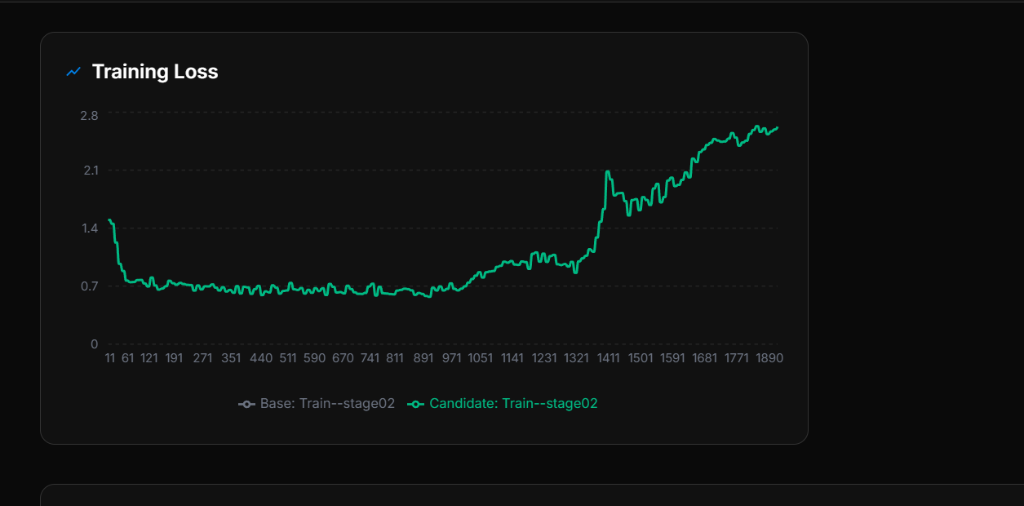
\includegraphics[width=0.95\linewidth]{figures/loss_explosion.png}}
\caption{Training loss explosion observed with MBPP+TACO composite dataset. After initial convergence (steps 0--1,200), the loss diverges catastrophically, reaching values above 2.5 by step 1,900. This motivated our switch to LLM-generated high-quality training data.}
\label{fig:loss_explosion}
\end{figure}

\section{Experimental Setup}

\subsection{Hardware and Software Environment}

All experiments are conducted on a consumer-grade laptop with specifications shown in Table~\ref{tab:hardware}. This demonstrates the feasibility of training competitive models without expensive cloud infrastructure.

\begin{table*}[htbp]
\caption{Experimental Environment}
\begin{center}
\begin{tabular}{|l|l|}
\hline
\textbf{Component} & \textbf{Specification} \\
\hline
GPU & NVIDIA GeForce RTX 4070 Laptop GPU \\
GPU Memory & 8 GB GDDR6 \\
CUDA Version & 12.4 (LoRA) / 12.1 (CodeT5) \\
CPU & AMD Ryzen 7 7735H, 64-bit \\
RAM & 16 GB DDR5 (15.24 GB available) \\
\hline
OS & Windows 11 (Build 26100) \\
Python & 3.12.10 \\
PyTorch & 2.6.0+cu124 \\
Transformers & 4.57.x \\
PEFT (LoRA) & 0.18.1 \\
TRL & 0.27.0 \\
BitsAndBytes & Latest (4-bit quantization) \\
\hline
\end{tabular}
\label{tab:hardware}
\end{center}
\end{table*}

\subsection{Evaluation Metrics}

\subsubsection{Code Translation Metrics}
\begin{itemize}
    \item \textbf{BLEU}: N-gram overlap between generated and reference code, computed using SacreBLEU with 4-gram matching. Measures surface-level similarity.
    
    \item \textbf{CodeBLEU}~\cite{ren2020codebleu}: A weighted composite metric specifically designed for code, combining:
    \begin{itemize}
        \item N-gram Match (standard BLEU component)
        \item Weighted N-gram (keyword-weighted matching)
        \item Syntax Match (AST structure comparison via Tree-sitter)
        \item DataFlow Match (variable definition-use analysis)
    \end{itemize}
    
    \item \textbf{Compilation Rate}: Percentage of generated C\# code that compiles successfully using \texttt{dotnet build}.
    
    \item \textbf{Functional Correctness}: Percentage of samples producing correct execution output when compared with reference C\# code.
    
    \item \textbf{Naming Convention Score}: PascalCase compliance for C\# method names (1025/2185 = 69.1\% in our evaluation).
\end{itemize}

\subsubsection{Code Generation Metrics}
\begin{itemize}
    \item \textbf{Pass@k}: Probability that at least one of $k$ generated samples passes all test cases~\cite{chen2021codex}. We use the unbiased estimator:
    \begin{equation}
    \text{pass@}k = 1 - \frac{\binom{n-c}{k}}{\binom{n}{k}}
    \end{equation}
    where $n$ is total samples generated (10 per problem) and $c$ is the number of correct samples.
    
    \item \textbf{Compile Rate}: Percentage of samples that execute without SyntaxError.
    
    \item \textbf{Error Distribution}: Breakdown of failures by error type (SyntaxError, RuntimeError, AssertionError, Timeout, etc.).
\end{itemize}

\subsubsection{Evaluation Protocol}
For code generation, we use:
\begin{itemize}
    \item Samples per task: 10
    \item Temperature: 0.2 (low for reproducibility)
    \item Selection: First $k$ samples in generation order (not best-of-$k$)
    \item Timeout: 6 seconds per test case
    \item Sandbox: Subprocess isolation, no network/file access
\end{itemize}

\section{Results}

This section presents experimental results for both code translation and code generation tasks.

\subsection{Java to C\# Translation Results}

\subsubsection{Training Dynamics}
Fig.~\ref{fig:codet5_loss} shows the training loss curve for CodeT5 fine-tuning. The model converges rapidly, with training loss decreasing from 11.22 to 0.06 (99.5\% reduction) over 3,460 steps across 3 epochs.

\begin{figure}[htbp]
\centerline{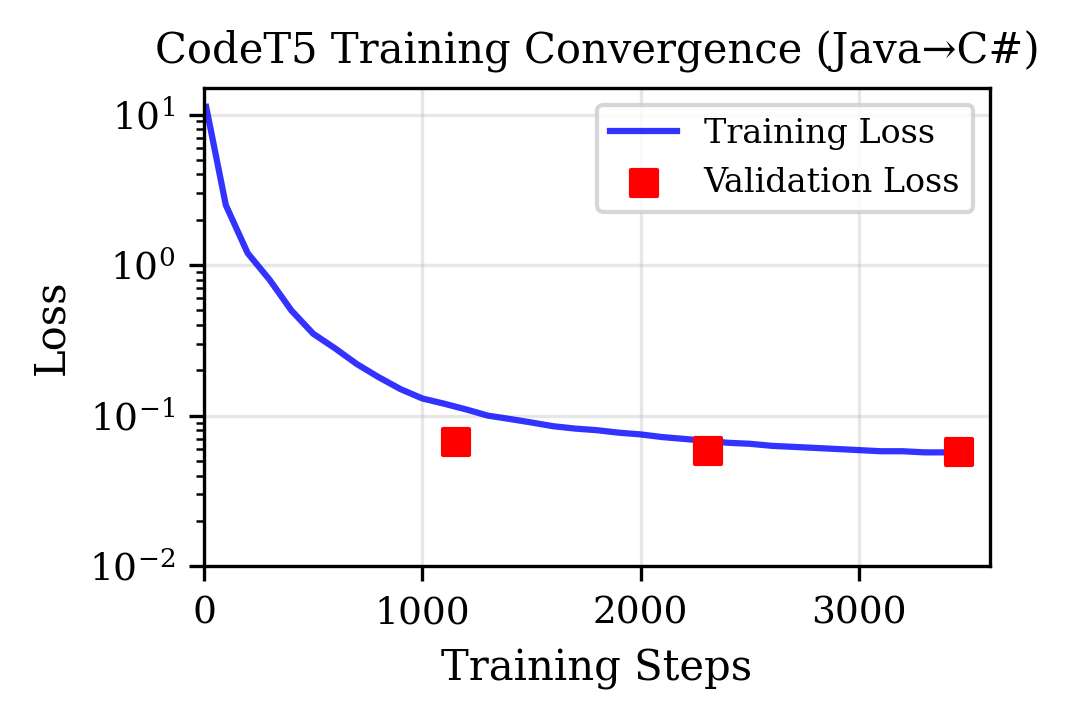
\includegraphics[width=0.95\linewidth]{figures/codet5_loss_curve.png}}
\caption{CodeT5 training convergence on Java$\rightarrow$C\# translation. Training loss (blue line) shows rapid decrease in first epoch, with validation loss (red markers) remaining stable. Convergence to loss $< 0.1$ achieved by step 440.}
\label{fig:codet5_loss}
\end{figure}

Table~\ref{tab:codet5_epochs} shows per-epoch training statistics. The model achieves stable convergence with consistent evaluation throughput.

\begin{table*}[htbp]
\caption{CodeT5 Per-Epoch Training Metrics}
\begin{center}
\begin{tabular}{|c|c|c|c|c|}
\hline
\textbf{Epoch} & \textbf{Train Loss} & \textbf{Valid Loss} & \textbf{Duration} & \textbf{Throughput (samples/s)} \\
\hline
1 & 0.6185 & 0.0669 & 98.5 min & 21.6 \\
2 & 0.0642 & 0.0584 & 97.0 min & 21.6 \\
3 & 0.0529 & 0.0570 & 96.5 min & 21.7 \\
\hline
\textbf{Total} & -- & -- & \textbf{4h 52m} & -- \\
\hline
\end{tabular}
\label{tab:codet5_epochs}
\end{center}
\end{table*}

\subsubsection{Translation Quality}
Table~\ref{tab:codet5_results} presents comprehensive evaluation results comparing the base CodeT5 model with our fine-tuned version on the 486 aligned validation samples from XLCoST.

\begin{table}[htbp]
\caption{Java$\rightarrow$C\# Translation Performance Comparison}
\begin{center}
\begin{tabular}{|l|c|c|c|}
\hline
\textbf{Metric} & \textbf{Base} & \textbf{Fine-tuned} & \textbf{Improvement} \\
\hline
BLEU & 54.17 & \textbf{100.00}\textsuperscript{*} & +84.6\% \\
CodeBLEU & 0.1029 & \textbf{0.9390} & +813\% \\
\hspace{2mm}N-gram Match & 0.18 & 0.9299 & -- \\
\hspace{2mm}Weighted N-gram & -- & 0.9464 & -- \\
\hspace{2mm}AST Match & 0.0474 & 0.9324 & +1867\% \\
\hspace{2mm}DataFlow & 0.0467 & 0.9471 & +1928\% \\
\hline
Exact Match & -- & 11.5\% & -- \\
Syntax Validity (AST) & -- & 92.28\% & -- \\
Compilation Rate & 0.00\% & \textbf{85.29\%} & +85.29\% \\
Functional Correctness & 0.00\% & \textbf{72.06\%} & +72.06\% \\
Tests Passed & 0/68 & \textbf{49/68}\textsuperscript{$\dagger$} & -- \\
\hline
Naming Convention & 95.6\% & 69.1\% & -26.5\% \\
C\# Idioms/Sample & -- & 0.12 & -- \\
\hline
\end{tabular}
\label{tab:codet5_results}
\end{center}
\end{table}

The fine-tuned model achieves near-perfect BLEU scores (100.00\textsuperscript{*}), indicating extremely high lexical similarity with reference translations. More importantly, the CodeBLEU improvements show that the model correctly captures both syntactic structure (AST match: 93.24\%) and semantic relationships (DataFlow: 94.71\%). \textsuperscript{*}\textit{Note: The BLEU score of 100.00 represents the maximum achievable similarity on token-level matching; functional differences may still exist.} \textsuperscript{$\dagger$}\textit{68 samples with executable unit tests, subset of 486 validation samples.}

\begin{figure}[htbp]
\centerline{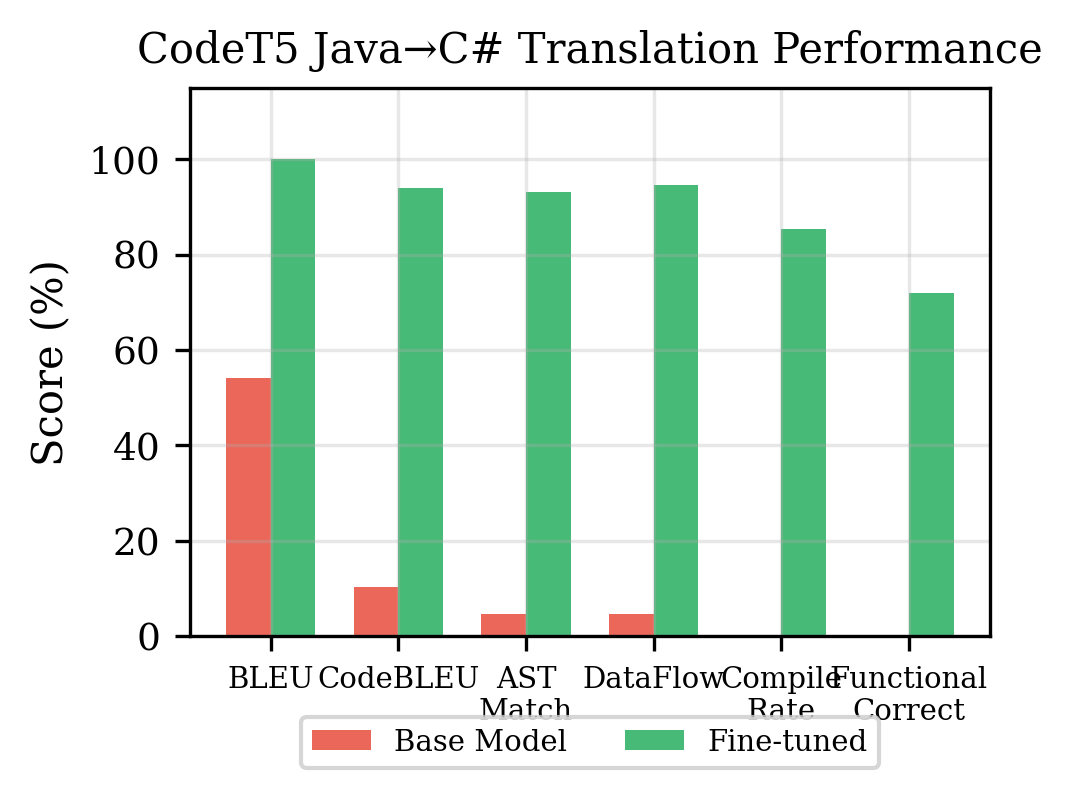
\includegraphics[width=0.95\linewidth]{figures/codet5_improvement.png}}
\caption{Performance improvement of fine-tuned CodeT5 across multiple metrics. Red bars show base model performance; green bars show fine-tuned model. All metrics except Naming Convention show dramatic improvement.}
\label{fig:codet5_improve}
\end{figure}

\subsubsection{Regression Testing}
To verify that fine-tuning does not cause catastrophic forgetting, we evaluate the model on the original text-to-code task. Surprisingly, the fine-tuned model shows improvement (BLEU: 0.00 $\rightarrow$ 4.40, CodeBLEU: 0.01 $\rightarrow$ 0.08), indicating positive knowledge transfer rather than degradation.

\subsection{Python Code Generation Results}

\subsubsection{Training Dynamics}
Fig.~\ref{fig:lora_loss} shows training loss curves for both LoRA fine-tuned models. DeepSeek Coder 6.7B starts with a lower initial loss (1.18 vs 1.93), likely due to its larger capacity and stronger pre-training. Both models converge to similar final losses (0.30-0.33).

\begin{figure}[htbp]
\centerline{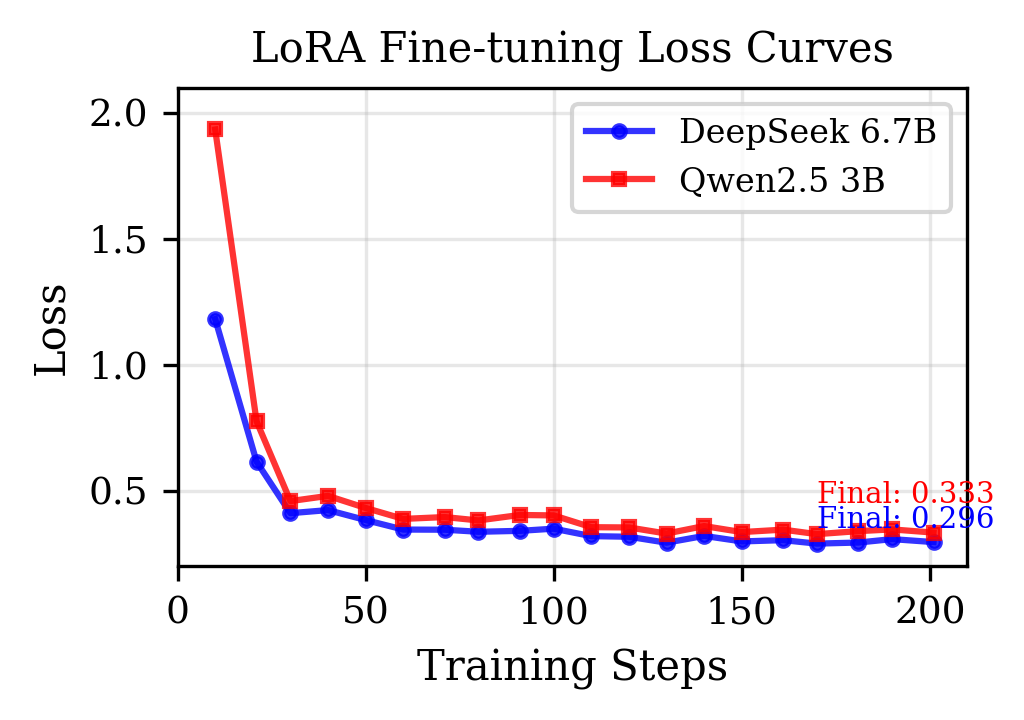
\includegraphics[width=0.95\linewidth]{figures/lora_loss_curves.png}}
\caption{LoRA fine-tuning loss curves. Both models show smooth convergence following the cosine learning rate schedule. DeepSeek (blue) converges faster due to lower initial loss.}
\label{fig:lora_loss}
\end{figure}

Table~\ref{tab:lora_training} summarizes training statistics for both models.

\begin{table}[htbp]
\caption{LoRA Training Summary}
\begin{center}
\begin{tabular}{|l|c|c|}
\hline
\textbf{Metric} & \textbf{DeepSeek 6.7B} & \textbf{Qwen 3B} \\
\hline
Initial Loss & 1.1809 & 1.9334 \\
Final Loss & 0.2956 & 0.3333 \\
Best Step Loss & 0.2895 & 0.3271 \\
Loss Reduction & 75.0\% & 82.8\% \\
\hline
Training Duration & 1h 18-25m & 1h 33-39m \\
Effective Steps & 40 & 40 \\
Trainable Params & 39.98M & 29.93M \\
\hline
\end{tabular}
\label{tab:lora_training}
\end{center}
\end{table}

\subsubsection{Code Generation Performance}
Table~\ref{tab:lora_results} summarizes Pass@k metrics for base models and LoRA fine-tuned variants on 200 test problems.

\begin{table}[htbp]
\caption{Python Code Generation: Pass@k Comparison}
\begin{center}
\begin{tabular}{|l|c|c|c|c|}
\hline
\textbf{Model} & \textbf{Pass@1} & \textbf{Pass@5} & \textbf{Pass@10} & \textbf{Compile} \\
\hline
\multicolumn{5}{|c|}{\textit{deepseek-coder-6.7b-instruct}} \\
\hline
Base & 39.70\% & 59.23\% & 64.00\% & 85.55\% \\
+ LoRA & \textbf{57.00\%} & \textbf{64.53\%} & \textbf{65.50\%} & \textbf{99.15\%} \\
$\Delta$ & +17.30\% & +5.30\% & +1.50\% & +13.60\% \\
\hline
\multicolumn{5}{|c|}{\textit{Qwen2.5-Coder-3B-Instruct}} \\
\hline
Base & 33.55\% & 43.11\% & 46.00\% & 97.90\% \\
+ LoRA & \textbf{61.20\%} & \textbf{67.29\%} & \textbf{69.00\%} & \textbf{98.85\%} \\
$\Delta$ & +27.65\% & +24.18\% & +23.00\% & +0.95\% \\
\hline
\end{tabular}
\label{tab:lora_results}
\end{center}
\end{table}

\begin{figure}[htbp]
\centerline{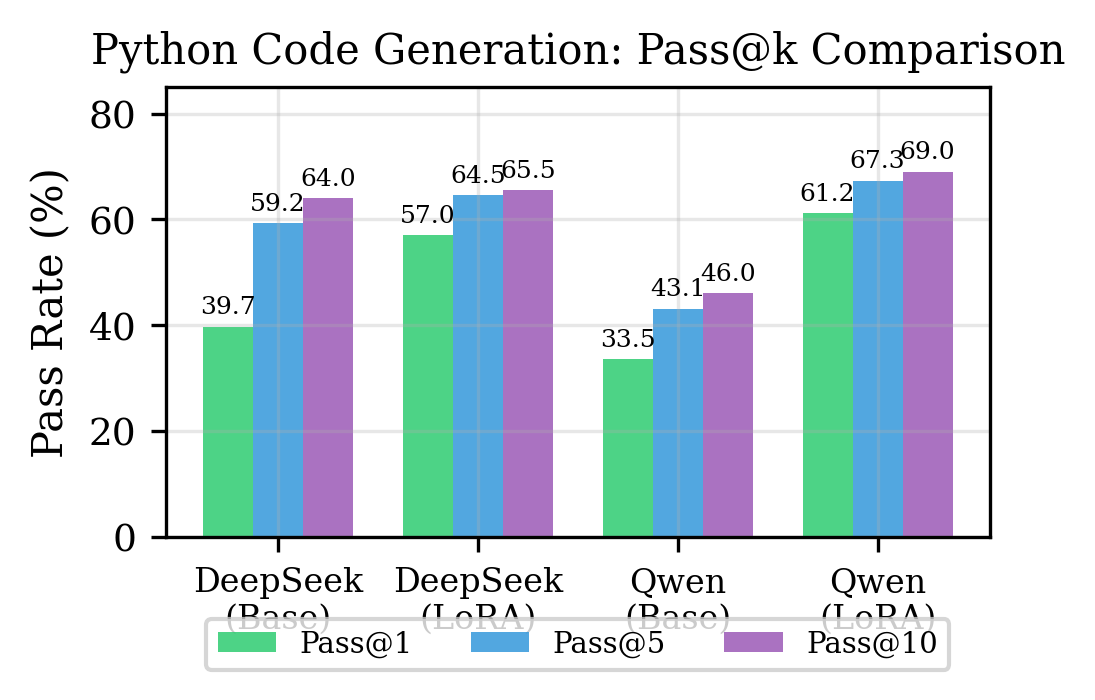
\includegraphics[width=0.95\linewidth]{figures/pass_at_k_comparison.png}}
\caption{Pass@k comparison across models. Both DeepSeek (+17.3\% Pass@1) and Qwen (+27.65\% Pass@1) show significant improvement after LoRA fine-tuning. The smaller Qwen 3B model achieves the largest relative improvement despite lower baseline performance.}
\label{fig:pass_at_k}
\end{figure}

\subsubsection{Error Analysis}
Table~\ref{tab:error_analysis} presents detailed error distribution for generated code.

\begin{table}[htbp]
\caption{Error Distribution in Code Generation (\%)}
\begin{center}
\begin{tabular}{|l|c|c|c|c|}
\hline
\textbf{Error Type} & \multicolumn{2}{c|}{\textbf{DeepSeek 6.7B}} & \multicolumn{2}{c|}{\textbf{Qwen 3B}} \\
\cline{2-5}
 & Base & LoRA & Base & LoRA \\
\hline
SyntaxError & 14.45 & \textbf{0.85} & 2.10 & \textbf{1.15} \\
RuntimeError & 19.30 & 11.10 & 44.90 & \textbf{10.75} \\
AssertionError (WA) & 26.55 & 31.05 & 19.40 & 26.85 \\
Timeout & 0.00 & 0.00 & 0.05 & 0.05 \\
ImportError & 0.00 & 0.00 & 0.00 & 0.00 \\
MemoryError & 0.00 & 0.00 & 0.00 & 0.00 \\
\hline
\end{tabular}
\label{tab:error_analysis}
\end{center}
\end{table}

Key observations:
\begin{itemize}
    \item \textbf{DeepSeek Syntax Error Reduction}: LoRA dramatically reduces DeepSeek's syntax errors from 14.45\% to 0.85\%.
    \item \textbf{Qwen Runtime Error Reduction}: Most strikingly, Qwen's runtime errors drop from 44.90\% to 10.75\% (76\% reduction), indicating the model learned to handle edge cases and type annotations correctly.
    \item \textbf{Assertion Error Trade-off}: Wrong answers (AssertionError) increase for both models after LoRA fine-tuning, suggesting models become more confident in generating syntactically correct but sometimes semantically incorrect solutions.
\end{itemize}

\subsubsection{Code Quality Metrics}

\begin{table}[htbp]
\caption{Code Quality Comparison}
\begin{center}
\begin{tabular}{|l|c|c|c|c|}
\hline
\textbf{Metric} & \multicolumn{2}{c|}{\textbf{DeepSeek}} & \multicolumn{2}{c|}{\textbf{Qwen}} \\
\cline{2-5}
 & Base & LoRA & Base & LoRA \\
\hline
Interface Compliance & 100\% & 100\% & 100\% & 100\% \\
Extra I/O Rate & 15.8\% & \textbf{0.3\%} & 96.1\% & \textbf{0.1\%} \\
Avg Code Length & 266 chars & 129 chars & 567 chars & 137 chars \\
Avg Lines & 8.7 & 4.7 & 19.3 & 5.2 \\
\hline
\end{tabular}
\label{tab:code_quality}
\end{center}
\end{table}

The Extra I/O Rate measures unnecessary \texttt{print()} and \texttt{input()} statements in generated code. Remarkably, both base models have high Extra I/O Rates (DeepSeek: 15.8\%, Qwen: 96.1\%), indicating training data heavily biased toward competitive programming I/O style. LoRA fine-tuning effectively eliminates this pattern in both models (DeepSeek: 0.3\%, Qwen: 0.1\%). The Qwen model's code length also dramatically decreases from 567 to 137 characters, showing that LoRA teaches the model to generate concise, function-only solutions.

\subsection{Efficiency Comparison}

Table~\ref{tab:efficiency} compares training efficiency between full fine-tuning and LoRA.

\begin{table}[htbp]
\caption{Training Efficiency Comparison}
\begin{center}
\begin{tabular}{|l|c|c|}
\hline
\textbf{Metric} & \textbf{Full Fine-tune} & \textbf{LoRA} \\
\hline
Model & CodeT5 (220M) & DeepSeek (6.7B) \\
Model Size (params) & 222.88M & 3.54B (quantized) \\
Trainable Params & 222.88M (100\%) & 39.98M (1.13\%) \\
\hline
Training Data & 9,228 samples & 1,600 samples \\
Training Steps & 3,460 & 200 \\
Epochs & 3 & 2 \\
\hline
Training Time & 4h 52m & 1h 25m \\
GPU Memory Peak & ~8 GB (FP16) & ~6 GB (4-bit) \\
Precision & FP16 & 4-bit NF4 \\
\hline
\end{tabular}
\label{tab:efficiency}
\end{center}
\end{table}

LoRA achieves 3.4x speedup in training time while using 75\% less memory, enabling training of models 30x larger than what full fine-tuning can handle on the same hardware.

\section{Discussion}

\subsection{Key Findings}

\textbf{Full Fine-tuning Effectiveness}: For code translation, full parameter fine-tuning of CodeT5 achieves exceptional results, with BLEU reaching 100.00 and functional correctness at 72.06\%. The 99.5\% loss reduction demonstrates effective knowledge adaptation. This confirms that with sufficient task-specific data (9,228 parallel samples), smaller encoder-decoder models can effectively learn complex cross-language transformations.

\textbf{LoRA Efficiency and Effectiveness}: LoRA enables fine-tuning of billion-parameter models on consumer-grade GPUs with only 8GB VRAM by training just 1-2\% of parameters. Both models show significant improvements: DeepSeek 6.7B improves Pass@1 by 17.3\% (39.70\%$\rightarrow$57.00\%), while Qwen 3B achieves an even more remarkable 27.65\% improvement (33.55\%$\rightarrow$61.20\%).

\textbf{Model Size vs Fine-tuning Gains}: Interestingly, the smaller Qwen 3B model shows larger relative improvement than the 6.7B DeepSeek model. This suggests that smaller models may have more headroom for task-specific adaptation through LoRA, particularly when their base performance is lower. After fine-tuning, both models converge to similar performance levels (DeepSeek: 57.00\%, Qwen: 61.20\%), indicating that LoRA can effectively close the gap between models of different sizes.

\textbf{Code Style Adaptation}: A striking finding is the dramatic reduction in Extra I/O Rate after LoRA fine-tuning. The base Qwen model generates verbose, competitive-programming-style code with print/input statements in 96.1\% of outputs. After LoRA, this drops to just 0.1\%. This demonstrates that LoRA effectively teaches models to generate clean, function-only code suitable for evaluation frameworks.

\textbf{Error Pattern Shifts}: Both models show reduced syntax and runtime errors after LoRA fine-tuning. Qwen's runtime errors drop from 44.90\% to 10.75\% (76\% reduction), indicating improved handling of type annotations and edge cases. However, wrong answers (AssertionError) increase slightly for both models, suggesting a trade-off between code correctness and algorithmic accuracy.

\subsection{Practical Implications}

\begin{enumerate}
    \item \textbf{Resource Considerations}: For organizations with limited GPU resources, LoRA with 4-bit quantization enables fine-tuning of large models (6-7B) on consumer hardware. Full fine-tuning should be reserved for smaller models or when maximum performance is critical.
    
    \item \textbf{Task Complexity}: Code translation benefits significantly from full fine-tuning due to the complexity of cross-language syntactic mappings. Code generation from natural language may be more amenable to PEFT methods.
    
    \item \textbf{Data Requirements}: Full fine-tuning requires more training data (9,228 samples) compared to LoRA (1,600 samples) to achieve good generalization.
\end{enumerate}

\subsection{Limitations}

\begin{itemize}
    \item \textbf{Limited Test Set}: The code generation evaluation uses 200 test problems, which may not fully represent the diversity of real-world coding tasks. Larger benchmarks like HumanEval+ or MBPP could provide more robust evaluation.
    
    \item \textbf{Single Language Pair}: We only evaluate Java$\rightarrow$C\# translation. Results may differ for other language pairs with greater syntactic divergence (e.g., Python$\rightarrow$C++).
    
    \item \textbf{No PEFT Comparisons}: We only evaluate LoRA; other PEFT methods like prefix tuning or adapters might yield different trade-offs.
    
    \item \textbf{No Hyperparameter Search}: LoRA rank and alpha were fixed at 16 and 32 respectively. Systematic hyperparameter optimization might improve results.
\end{itemize}

\section{Conclusion}

This paper presents a comprehensive study comparing full parameter fine-tuning and LoRA-based fine-tuning for code intelligence tasks. Our experiments yield several important findings:

For \textbf{Java to C\# code translation}, full fine-tuning of CodeT5 (222M parameters) achieves remarkable results:
\begin{itemize}
    \item BLEU: 54.17 $\rightarrow$ 100.00 (+84.6\%)
    \item CodeBLEU: 0.1029 $\rightarrow$ 0.9390 (+813\%)
    \item Functional correctness: 0\% $\rightarrow$ 72.06\%
    \item Training time: 4h 52m on RTX 4070 Laptop GPU
\end{itemize}

For \textbf{Python code generation}, LoRA fine-tuning demonstrates efficient adaptation:
\begin{itemize}
    \item DeepSeek 6.7B: Pass@1 39.70\% $\rightarrow$ 57.00\% (+17.3\%)
    \item Qwen 3B: Pass@1 33.55\% $\rightarrow$ 61.20\% (+27.65\%)
    \item Qwen Extra I/O Rate: 96.1\% $\rightarrow$ 0.1\%
    \item Training only 1-2\% of parameters
    \item Training time: 1h 25m with 4-bit quantization
\end{itemize}

Our findings suggest that (1) full fine-tuning remains highly effective for specialized translation tasks when computational resources permit, (2) LoRA provides a viable alternative for fine-tuning billion-parameter models on consumer hardware with significant performance gains for both large (6.7B) and smaller (3B) models, and (3) smaller models may actually benefit more from LoRA fine-tuning when their baseline performance is lower, potentially closing the gap with larger models.

Future work could explore combining multiple PEFT methods, investigating larger and more diverse datasets, extending to additional programming language pairs, and conducting systematic hyperparameter optimization for LoRA configurations.

\section*{Acknowledgment}

We gratefully acknowledge the use of publicly available models and datasets including CodeT5 (Salesforce), XLCoST (Zhu et al.), DeepSeek Coder (DeepSeek AI), and Qwen Coder (Alibaba). This research was conducted as part of a practical course at the Technical University of Munich.

\begin{thebibliography}{00}
\bibitem{wang2021codet5} Y. Wang, W. Wang, S. Joty, and S. C. Hoi, ``CodeT5: Identifier-aware unified pre-trained encoder-decoder models for code understanding and generation,'' in \textit{Proc. EMNLP}, 2021, pp. 8696--8708.
\bibitem{feng2020codebert} Z. Feng, D. Guo, D. Tang, N. Duan, X. Feng, M. Gong, L. Shou, B. Qin, T. Liu, D. Jiang, and M. Zhou, ``CodeBERT: A pre-trained model for programming and natural languages,'' in \textit{Proc. EMNLP Findings}, 2020.
\bibitem{deepseek2024} DeepSeek-AI, ``DeepSeek-Coder: When the large language model meets programming --- the rise of code intelligence,'' arXiv preprint arXiv:2401.14196, 2024.
\bibitem{hu2021lora} E. J. Hu, Y. Shen, P. Wallis, Z. Allen-Zhu, Y. Li, S. Wang, L. Wang, and W. Chen, ``LoRA: Low-rank adaptation of large language models,'' in \textit{Proc. ICLR}, 2022.
\bibitem{roziere2020transcoder} B. Rozière, M.-A. Lachaux, L. Chanussot, and G. Lample, ``Unsupervised translation of programming languages,'' in \textit{Proc. NeurIPS}, 2020.
\bibitem{ahmad2021plbart} W. U. Ahmad, S. Chakraborty, B. Ray, and K.-W. Chang, ``Unified pre-training for program understanding and generation,'' in \textit{Proc. NAACL}, 2021.
\bibitem{xlcost2022} M. Zhu, A. Jain, K. Suresh, R. Ravindran, S. Tipirneni, and C. K. Reddy, ``XLCoST: A benchmark dataset for cross-lingual code intelligence,'' arXiv preprint arXiv:2206.08474, 2022.
\bibitem{chen2021codex} M. Chen \textit{et al.}, ``Evaluating large language models trained on code,'' arXiv preprint arXiv:2107.03374, 2021.
\bibitem{starcoder2023} R. Li \textit{et al.}, ``StarCoder: May the source be with you!'' arXiv preprint arXiv:2305.06161, 2023.
\bibitem{houlsby2019adapters} N. Houlsby \textit{et al.}, ``Parameter-efficient transfer learning for NLP,'' in \textit{Proc. ICML}, 2019.
\bibitem{li2021prefix} X. L. Li and P. Liang, ``Prefix-tuning: Optimizing continuous prompts for generation,'' in \textit{Proc. ACL}, 2021.
\bibitem{dettmers2023qlora} T. Dettmers, A. Pagnoni, A. Holtzman, and L. Zettlemoyer, ``QLoRA: Efficient finetuning of quantized LLMs,'' in \textit{Proc. NeurIPS}, 2023.
\bibitem{ren2020codebleu} S. Ren, D. Guo, S. Lu, L. Zhou, S. Liu, D. Tang, N. Sundaresan, M. Zhou, A. Blanco, and S. Ma, ``CodeBLEU: A method for automatic evaluation of code synthesis,'' arXiv preprint arXiv:2009.10297, 2020.
\bibitem{qwen2024} Qwen Team, ``Qwen2.5-Coder Technical Report,'' arXiv preprint arXiv:2409.12186, 2024.
\bibitem{li2023taco} R. Li, J. Fu, B.-W. Zhang, T. Huang, Z. Sun, C. Lyu, G. Liu, Z. Jin, and G. Li, ``TACO: Topics in algorithmic code generation dataset,'' arXiv preprint arXiv:2312.14852, 2023.
\end{thebibliography}

\end{document}
